\section{Out of Order Execution}
Out of order execution is the key feature that Meltdown vulnerability exploits on Intel's micro-architectures. Basically, what
Meltdown does is possibile only because how Intel processors micro-architecture is designed.

Out of order is a technique used by almost every CPU both for Desktop and Server/Cloud machines, the main reason being the improvements on perfomance that it brings, allowing
CPU to execute instructions in a different order than how the program was compiled, in order to avoid wasting of computational power.
In this paper we refer to out-of-order as `out-of-order issue out-of-order completion'.

\subsubsection{Tomasulo's algorithm}
For a better understaindg of the Intel's CPU architecture, here is a brief introduction to Tomasulo's algorithm which
first introduced to techniques like register renaming, reservation station and common data bus (CDB), which allowed
out-of-order execution.

\begin{quote}
    In 1967, Tomasulo developed an algorithm that
    enabled dynamic scheduling of instructions to allow
    out-of-order execution.
\end{quote} [1]

Tomasulo's reservation station allows instructions that operate on the same physical registers to rename registers (register renaming), i.e. duplicating
register names in order to allow different instructions operate on the same register at the same time. This techinque solves read-after-write (True data dependeny, or RAW),
write-after-read (Antidependency, or WAR) and write-after-write (WAW) hazards.
Moreover, this lets the execution units use data values as soon as they are computed rather then reading value from a register,
writing the result on the register and then, again, reading it.
All execution units are directly (and individually) connected to the reservation station via a common data bus (CDB), where operands of instructions are
passed as soon as they're available. This is useful if an instruction is waiting for an operand that is not already on the register, so it can directly listen
on the CDB to recive the operand as soon as it is available.

\subsubsection{Intel Architecture}
Meltdown researchers provide a simplified illustration of a single core of the Intel's Skylake microarchitecture:

\begin{figure}
    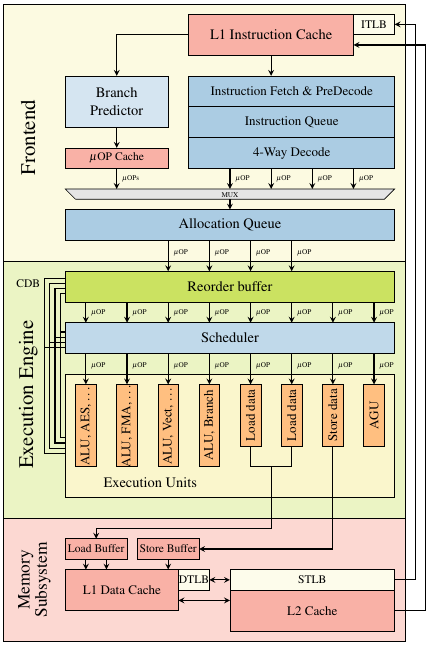
\includegraphics[scale=0.5]{img/skylake.png}
    \caption{Simplified illustration of a single core of the Intel's Skylake microarchitecture. Credits goes to Meltdown research team}
\end{figure}

The pipeline of Intel's Skylake processors consists of the front-end, which fetches instructions from memory and decodes them into micro-operations
(since intel's processors are CISC, while Superscalar/superpipelined processors suits better on RISC, the processor must decode complex operations
into smaller, less complex micro-operations in order to leverage out-of-order execution), the back-end (execution engine), which implements
out-of-order execution, and the memory subsystem.
The Reorder Buffer is responsible of register allocation, register renaming and retiring (reordering instruction outputs
as was intended by the program(mer)).
Micro-operations are directly forwarded to the Unified Reservation Station that queues the operations on exit ports that are connected to Execution Units.
Of course, Intel's Skylake has it's branch predictor. Usally branch predictors are implemented with \textit{taken/not taken} bits which tracks the history
of a branch and indicates if previosly the branch was taken or not taken. This can be implemented with 1-bit or 2-bit counters. More on this on Branch Predictiors section.

\subsubsection{How Meltdown leverages Reservation Station on Intel's micro-architecture}
Since out-of-order execution allows the processor to execute instructions before previous instructions have effectivily terminated their tasks, it is impossibile
for the processor to verify if any of the instructions that should be executed before raises an exception, e.g. access to a memory address where the program
should not be able to, Meltdown leverages exactly this concept with transient instructions computing data that the program should not be able to access. More on this
on the Meltdown chapter.

